\documentclass[11pt, frenchb]{article}
\usepackage[utf8]{inputenc}
\usepackage[T1]{fontenc}
\usepackage[french]{babel}
\usepackage{amsmath}
\usepackage[bookmarks={true},bookmarksopen={true}]{hyperref}
\usepackage{graphicx}
\usepackage[a4paper]{geometry}
\usepackage{listings}
	\lstset{frame=tb,
		language=Java,
 		aboveskip=3mm,
  		belowskip=3mm,
  		showstringspaces=false,
  		columns=flexible,
  		basicstyle={\small\ttfamily},
  		numbers=none,
 		numberstyle=\tiny\color{gray},
  		keywordstyle=\color{blue},
  		commentstyle=\color{dkgreen},
  		stringstyle=\color{mauve},
  		breaklines=true,
  		breakatwhitespace=true
  		tabsize=3
	}
\pagestyle{plain}
\setlength{\parindent}{5mm}
\usepackage{amsmath}
\usepackage{color}

\definecolor{dkgreen}{rgb}{0,0.6,0}
\definecolor{gray}{rgb}{0.5,0.5,0.5}
\definecolor{mauve}{rgb}{0.58,0,0.82}



\title{\textbf{Projet LSINF1121 -  Algorithmique et structures de données\\ - \\ Rapport final Mission 4} \\ {\large Groupe 26}}
\author{Laurian \bsc{Detiffe} \\(6380-12-00)\and Sundeep \bsc{Dhillon} \\(6401-11-00)\and Alexis \bsc{Macq} \\ (5910-12-00) \and Xavier \bsc{Pérignon} \\ (8025-11-00)\and Thibaut \bsc{Piquard}\\(4634-13-00)\and Thomas \bsc{Wyckmans} \\ (3601-12-00)}
\date{date}
\date{\vspace*{25mm}

\includegraphics[scale=0.75]{logo.jpg}\\
		\vspace*{30mm}
		\begin{center}
		Année académique 2015-2016 \\	
		\end{center}}

\begin{document}
\thispagestyle{empty}

\maketitle
\thispagestyle{empty}
%\tableofcontents
%\setcounter{tocdepth}{3}
%\setcounter{page}{1}
%\newpage

\section*{Introduction}
Dans le cadre de cette quatrième mission, nous avons eu pour but de réaliser un programme permettant de détecter du plagiat via l'algorithme de Rabin-Karp et ce, en implémentant notre propre HashMap.

\section{Constructeur de Plagiarism}
Le constructeur de la classe Plagiarism prend en argument un string indiquant le chemin vers le dossier où se trouvent les fichiers à comparer ainsi que un int indiquant le nombres minimal de caractères qui doivent correspondre entre ces documents et le fichier de base pour qu'on puisse considérer du plagiat (nous les nommerons W) . Notre constructeur implémente un tableau d'éléments de type file en utilisant la méthode ".listFiles()" afin de récupérer tous les chemins pour les fichiers compris dans le dossier mis en argument.

\section{Méthode create}
La fonction create de la classe Plagiarism prend en argument un string contenant le chemin vers un fichier et renvoie une HashMap contenant des clés représentant des strings de W chars . La méthode commence tout d'abord par un try/catch permettant de gérer le FileNotFoundException. Dans celui-ci, on initialise un scanner qui lira l'entièreté du Fichier et le convertira sous forme d'un long string.\\
Ensuite, on utilise une boucle for pour pour remplir le Hashmap à l'aide de substring. La première insertion se fait d'abord en complexité O(k) puis ensuite elle passe en O(1) grâce à la méthode incrementalHashCode().

\section{Constructeur de HashMap}
Pour résoudre les problèmes de collisions de notre HashMap, nous utilisons les propriétés du "linear probing". Cette structure permet de mapper un String avec un Integer.

\section{Fonction hashCode}
La fonction de hashage utilise une méthode de Horner et cela afin de pouvoir implémenter la fonction incrementalHashCode avec la complexité voulue.\\
Cette fonction calcul le hash associé au String passé en argument. Elle utilise la fonction getNumericValue de la librairie Character afin de faire la conversion entre les caractères et les int. Cela implique que les int passés en argument de la fonction incrementalHashCode doivent aussi être des caractères transformés en int via la fonction getNumericValue.

\section{Fonction incrementalHashCode}
Cette fonction calcul le hash du mot décallé d'un caractère vers la droite sur base du hash précédent.\\
Par exemple, elle calcule le hash pour le mot "arginale" si vous lui donner la longueur des mots en cours (à savoir 8) en premier argument, la valeur numérique du premier caractère de marginal (à savoir celle de 'm') en deuxième argument, la valeur du hash du mot "marginal" en troisième argument et la valeur numérique du caractère "ajouté" en dernier argument.\\ 
Comme expliqué dans la section précédente, les int passés en argument de la fonction incrementalHashCode doivent être des caractères transformés en int via la fonction getNumericValue.\\
Cette fonction utilise le fait que la fonction hashCode utilise une méthode de Horner.\\Cela lui permet de retirer la contribution de la première lettre du mot précédent au hash du mot précédent et de lui ajouté la contribution du nouveau caractère afin d'obtenir le nouveau hash.\\
Cela se fait aisément sur base du raisonnement suivant :\\
La méthode utilisé pour le Hash implique que le string $ s[i,..., i+n-1] = t_i*R^{n-1} + t_{i+1}*R^{n-2}+...+t_{i+n-1}*R^0 $ quand il est découpé par la méthode de Horner.\\
(Il faut après cela bien sûr fair un modulo de cette valeur via un nombre premier 
mais nous ne détaillerons pas les calculs supplémentaires dus au modulo. Ceux-ci se basent sur la propriété suivante des modulos :\\
$$ (a+b)\,\bmod\,n = ((a\,\bmod\,n)+(b\,\bmod\,n))\,\bmod\,n $$
.)\\ 
On peut alors voir qu'on peut obtenir l'égalité suivante qui va nous permettre d'obtenir en une opération le hash du mot décallé sur base du hash du mot précédent une fois qu'on lui appliquera l'opération modulo adéquate : 
$$ x_{i+1} = (x_i - t_i * R^{n-1}) * R + t_{i+n} $$
Dans notre code cette opération a été séparée en deux une fois les opérations modulos appliquées. La première permettant de retirer la contribution du premier caractère et la deuxième d'ajouter celle du nouveau caractère. Pour la fonction hashCode() et incrementalHashCode(), nous utilisons le flag 0x7FFFFFFF afin de ne pas tomber sur un nombre négatif.
\newpage
\section{Améliorations}
Il existe deux améliorations que nous pouvons apporter à notre projet pour diminuer la complexité :
\begin{itemize}
\item utiliser la méthode Rabin-Karp dans nos fonctions HashMap afin de résoudre le problème du Substring Pattern Matching en $O(n + k)$ expected au lieu de $O(n * k)$.
\item construire une HashMap pour tous les documents du corpus et créer une méthode Comparable qui permettrait de comparer directement deux éléments dans deux HashMap distincts.
\end{itemize}

\section{Conclusion}
Notre code marche localement (testé avec l'exemple de l'ennoncé). Cependant, sa complexité n'est pas assez optimisée pour passer au travers du Timeout sur la plateforme INGInious.

\newpage
\section*{Annexe}
\begin{figure} [!h]
\centering
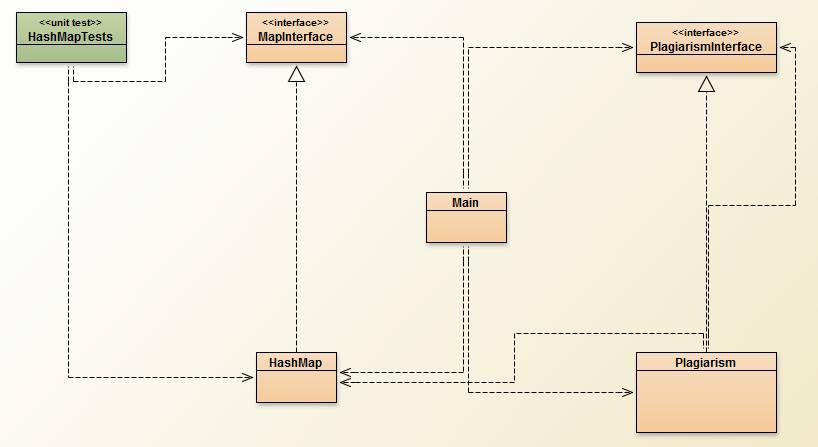
\includegraphics[scale=0.6]{diag.jpg}
\caption{Diagramme de classes}
\end{figure}
\end{document}